\documentclass[xcolor=svgnames]{beamer}
%\documentclass[xcolor=svgnames, handout]{beamer}

%\includeonlyframes{current}

\usepackage[utf8]    {inputenc}
\usepackage[T1]      {fontenc}
\usepackage[english] {babel}

\hypersetup{
     colorlinks = true,
     linkcolor = blue,
     anchorcolor = blue,
     citecolor = blue,
     filecolor = blue,
     urlcolor = blue
     }
     
\usepackage{amsmath,amsfonts,graphicx}
\usepackage{beamerleanprogress}
\usepackage{xcolor}
\usepackage{soul}
%\usepackage{verbatim}
\usepackage{multicol}
\usepackage{tikz} 
\usepackage[export]{adjustbox}

\usepackage{fancyvrb}
\usepackage{spverbatim}

\usepackage{xcolor}

\definecolor{iyellow}{RGB}{255, 162, 23}
\definecolor{sgreen}{RGB}{118, 191, 138}

\newcommand{\yellow}[1]{\textcolor{iyellow}{#1}}
\newcommand{\red}[1]{\textcolor{red}{#1}}
\newcommand{\green}[1]{\textcolor{ForestGreen}{#1}}
\newcommand{\blue}[1]{{\textcolor{blue}{#1}}}
\newcommand{\orange}[1]{{\textcolor{orange}{#1}}}
\newcommand{\bblue}[1]{\textcolor{SteelBlue!90!gray}{#1}} % beamer blue
\newcommand{\purple}[1]{{\textcolor{purple}{#1}}}


\newcommand{\el}{\\[1em]\pause}
\newcommand{\nl}{\\[1em]}
\newcommand{\define}[1]{\textbf{\textcolor{orange}{#1}}}
\newcommand{\answer}[1]{\textit{\textbf{\textcolor{iyellow}{#1}}}}
\newcommand{\command}[1]{\texttt{\textbf{\textcolor{DarkMagenta}{#1}}}}
\newcommand{\ipic}[2]{\includegraphics[width={#2}\textwidth]{#1}}
\newcommand{\cell}[1]{{\sf \textbf{\textcolor{DarkMagenta}{#1}}}}
\newcommand{\ra}{$\rightarrow$}

% timed answer
\newcommand{\tans}[2]{\textbf<#1>{\textit<#1>{{\color<#1>{iyellow}{#2}}}}}

\newcommand{\ft}[1]{\frametitle{#1}}

% for straight quotes in verbatim:
\usepackage{upquote,textcomp}

\usepackage[T1]{fontenc}
\usepackage[utf8]{inputenc}
\usepackage{tikz}
\usetikzlibrary{shadows}

\usepackage{upquote,textcomp}
\newenvironment{allintypewriter}{\ttfamily}{\par}
\newcommand{\bs}{$\backslash$}




\newcommand*\keystroke[1]{%
  \tikz[baseline=(key.base)]
    \node[%
      draw,
      fill=white,
      drop shadow={shadow xshift=0.25ex,shadow yshift=-0.25ex,fill=black,opacity=0.75},
      rectangle,
      rounded corners=2pt,
      inner sep=1pt,
      line width=0.5pt,
      font=\scriptsize\sffamily
    ](key) {#1\strut}
  ;
}

\title
  [Data 301 Data Analytics]
  {Data 301 Data Analytics\\
Python Data Analytics}

\author
  [Dr.\ Irene Vrbik]
  {Dr.\ Irene Vrbik}

\date
  {}

\institute
  {University of British Columbia Okanagan \newline irene.vrbik@ubc.ca}


\graphicspath{{img/}}

\begin{document}

\maketitle

\setbeamersize{description width=0.57cm} % to have less indent with the description environment




\begin{frame}[fragile]\ft{Python Modules}
%, commandchars=\\\{\}
{\textit Recall:}\\
A Python \emph{module} or library is code written by others for a specific purpose.  Whenever coding, make sure to look for modules that are already written for you to make your development faster!
Modules are imported using the import command:

\begin{Verbatim}[xleftmargin=.5in] 
import <modulename>
\end{Verbatim}

Useful modules for data analytics:
\begin{itemize}
\item {\tt Biopython} (bioinformatics), 
\item {\tt NumPy} (scientific computing/linear algebra), 
\item {\tt scikit-learn} (machine learning), 
\item {\tt pandas} (data structures), 
\item {\tt BeautifulSoup} (HTML/Web)
\end{itemize}
\end{frame}


\begin{frame}
[fragile]\ft{Biopython}
Biopython (\href{http://biopython.org}{see more here}) is a Python library for biological and bioinformatics computation.\nl

Features:
\begin{itemize}
\item parsers for bioinformatics file formats (BLAST, Clustalw, FASTA, Genbank)
\item access to online services (NCBI - National Center for Biotechnology Information)
\item sequence class
\item clustering/classification (k Nearest Neighbors, Naive Bayes, Support Vector Machines)
\item Integration with BioSQL (sequence database schema)
\end{itemize}
\end{frame}



\begin{frame}
[fragile]\ft{Biopython Installation}
Install in Anaconda by typing (in Command Line):
%, commandchars=\\\{\}
\begin{Verbatim}[xleftmargin=.5in] 
conda install biopython
\end{Verbatim}
Check if successfully installed and current version by typing (while running Python):
\begin{Verbatim}[xleftmargin=.5in] 
import Bio
print(Bio.__version__)
\end{Verbatim}
There are some useful resources: \href{http://biopython.org/DIST/docs/tutorial/Tutorial.html}{Biopython Tutorial and Cookbook},  and \href{https://biopython.org/wiki/Category%3AWiki_Documentation} {wiki documentation} on their \href{https://biopython.org/}{website}.
\end{frame}



\begin{frame}
[fragile]\ft{Biopython for FASTA files}
\begin{itemize}
\item Today we'll be using Biopython with FASTA files accessed through \href{https://www.ncbi.nlm.nih.gov/nuccore}{NCBI} website.
\item A FASTA files are text-based that follow a specific format for representing either nucleotide sequences or amino acid (protein) sequences.
\item Nucleotides or amino acids are represented using single-letter codes (eg A, T, C, G).
\item These files begin with a sing line description, followed by the lines of the sequence data.
\item New lines are distinguished by "\verb|>|"
\end{itemize}
\end{frame}


\begin{frame}
[fragile]\ft{Biopython for FASTA files}
\begin{center}
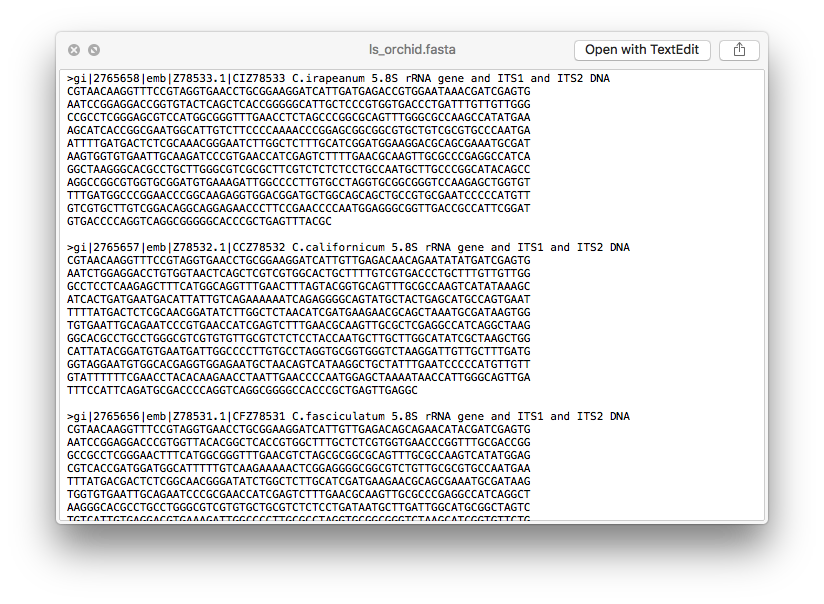
\includegraphics[width=0.99\textwidth]{img/fasta.png}
\end{center}
\end{frame}

\begin{frame}[fragile]\ft{Module IUPAC}
The International Union of Pure and Applied Chemistry (IUPAC)
\href{https://www.bioinformatics.org/sms/iupac.html}{notation} encodes nucleobases  by the first letters of their chemical names: \define Guanine,  \define Cytosine, \define Adenine, and \define Thymine.[1]\nl

Eleven "ambiguity" characters are used to encode every possible combination of the four DNA bases.  The use for them arises when  positional variations are found among families of related genes.\nl

The \verb|"IUPAC.unambiguous_dna"| specifies the ``\href{http://biopython.org/DIST/docs/api/Bio.Alphabet.IUPAC-module.html}{alphabet}" for the sequence\footnote{similar to {\tt string.ascii\_uppercase} providing the upper case alphabet.}
\begin{itemize}
\item Unambiguous DNA sequences will contain letters: A, C, G, T
\item Ambiguous DNA sequences will contain the letters: A, C, G, T,  R, Y, S, W, K, M, B, D, H, V, N
\end{itemize}
\end{frame}


\begin{frame}[fragile]\ft{Biopython Example - Using Sequences}
%, commandchars=\\\{\}
\begin{Verbatim}[commandchars=\\\{\}]
\purple{# Create a sequence from a string}
from Bio.Seq import Seq
my_seq = Seq("AGTACACTGGT")
\end{Verbatim}
Notice that this creates a new class of object called {\tt Bio.Seq.Seq} (or just {\tt Seq} object).
\begin{Verbatim}[frame=single]
>>> print(my_seq)
AGTACACTGGT
>>> print(type(my_seq))
<class 'Bio.Seq.Seq'>
>>> str_seq = "AGTACACTGGT"
>>> print(type(str_seq))
<class 'str'>
\end{Verbatim}


\end{frame}





\begin{frame}[fragile]
 The {\tt Bio.Seq} module allows us to make use of the sequence class type. \nl
 While sequences look just like strings on the surface, python will actually treat them differently.\nl
The {\tt Seq} object provides a number of string like methods (such as count, find, split and strip), which are alphabet aware where appropriate:
\begin{Verbatim}[frame=single]
>>> # find the length of the sequence:
>>> len(my_seq)
11
>>> # count the number of As that appear in the seq:
>>> my_seq.count("A")
3
\end{Verbatim}

\end{frame}


\begin{frame}
In addition there are some {\tt Seq} specific functions that we would not be able to apply to regular python strings. 
\begin{itemize}
\item  	
{\tt transcribe}
returns the RNA sequence from a DNA sequence by creating a new {\tt Seq} object.
\item eg. {\tt repr} return the (truncated) representation of the sequence for debugging.
\item eg. {\tt complement} return the complement sequence by creating a new Seq object.
%\item eg. {\tt len} return the length of the sequence.
\item see a list of functions \href{https://biopython.org/DIST/docs/api/Bio.Seq.Seq-class.html}{here}.
\end{itemize}

\end{frame}




\begin{frame}[fragile]\ft{Biopython Example - Using Sequences}
We can read in fasta files in a similar way to how we read regular text files.\nl
Namely, the {\tt SeqIO.parse()} function will open a connection to the fasta file, that we can then traverse through using a {\tt for} loop:
\begin{Verbatim}[commandchars=\\\{\}]
\purple{# Read a FASTA file and print sequence info}
from Bio import SeqIO
for seq_record in SeqIO.parse("sequence.fasta", "fasta"):
    print(seq_record.id)
    print(repr(seq_record.seq))
    print(len(seq_record))
    print(seq_record.seq.complement())
\end{Verbatim}
\end{frame}

%\begin{frame}
%[fragile]\ft{Biopython for FASTA files}
%\begin{itemize}
%\item 
%\end{itemize}
%\end{frame}


\begin{frame}
\ipic{img/dna}{0.9}

Picture taken from \href{https://www.khanacademy.org/science/biology/gene-expression-central-dogma/transcription-of-dna-into-rna/a/overview-of-transcription}{here}
\end{frame}






\begin{frame}[fragile]\ft{Biopython Transcription Example}
%, commandchars=\\\{\}
\begin{Verbatim}[commandchars=\\\{\}, fontsize=\small, frame=single]
# Transcription
from Bio.Seq import Seq
from Bio.Alphabet import IUPAC

coding_dna = Seq("TGCATTGGGTGCTGA",IUPAC.unambiguous_dna)
template_dna = \purple{coding_dna.reverse_complement()}
messenger_rna = \purple{coding_dna.transcribe()}

print("Coding:       ",coding_dna)
print("Template:     ",template_dna)
print("Messenger RNA:",messenger_rna)
print("Translation:  ",messenger_rna.translate())
\end{Verbatim}
Output:
\begin{Verbatim}[frame=single]
Coding:        TGCATTGGGTGCTGA
Template:      TCAGCACCCAATGCA
Messenger RNA: UGCAUUGGGUGCUGA
Translation:   CIGC*
\end{Verbatim}

\end{frame}


\begin{frame}[fragile]\ft{Biopython - Entrez Database Search}
\href{https://www.ncbi.nlm.nih.gov/Web/Search/entrezfs.html}{Entrez} is a federated database enabling retrieval of data from many  health sciences databases hosted by the NCBI.

%, commandchars=\\\{\}
\begin{Verbatim}[xleftmargin=.1in, fontsize=\small, commandchars=\\\{\}] 
# Retrieve data from nucleotide database as FASTA
\purple{from Bio import Entrez}
\purple{from Bio import SeqIO}
Entrez.email = "test@test.com"
# Providing GI for single entry lookup
\purple{handle = Entrez.efetch(db="nucleotide", rettype="fasta",} 
\purple{... retmode="text", id="3288717")}
record = SeqIO.read(handle, "fasta")
handle.close()
print(record)
\end{Verbatim}

\end{frame}



\begin{frame}[fragile]\ft{Biopython - BLAST}
\define{BLAST} (\define Basic \define Local \define Alignment \define Search \define Tool) compares an input sequence with database and returns similar sequences. See \href{http://blast.ncbi.nlm.nih.gov/}{here} 
%, commandchars=\\\{\}
\begin{Verbatim}[xleftmargin=.1in, frame=single] 
from Bio.Blast import NCBIWWW

sequence = "ACTATTCCAAACAGCTCATAACCAGAAA"
handle = NCBIWWW.qblast("blastn", "nt", sequence)
result = handle.read()
print(result)	# Output is in XML format
\end{Verbatim}
N.B.  The results are not instantaneous (may take a minute to run). Here is some output:
\begin{Verbatim}[frame=single, fontsize=\small]
<?xml version="1.0"?>
<!DOCTYPE BlastOutput PUBLIC "-//NCBI//NCBI BlastOutput/EN" "http://www.ncbi.nlm.nih.gov/dtd/NCBI_BlastOutput.dtd">
<BlastOutput>
  <BlastOutput_program>blastn</BlastOutput_program>
  ...
\end{Verbatim}

\end{frame}

\begin{frame}[fragile]\ft{Biopython - BLAST}
The  code from the previous slide essentially copy and pastes your sequence into the \href{https://blast.ncbi.nlm.nih.gov/Blast.cgi?PROGRAM=blastn&PAGE_TYPE=BlastSearch&LINK_LOC=blasthome}{NCBI web server} which  performs an algorithm for string matching.\nl
{\tt blastn} specifies the type of algorithm ({\tt n} for nucleotide) where {\tt nt}  (for nucleotide) gives the name of the database you want to search.\nl 

The query preformed by {\tt NCBIWWW.qblast} will open an XML  file that we can read from.\nl



\end{frame}


\begin{frame}[fragile]\ft{Biopython BLAST - Parsing Results}\label{intblast}
%
\begin{Verbatim}[xleftmargin=.1in, commandchars=\\\{\}, frame=single] 
from Bio.Blast import NCBIWWW \purple{# for BLAST request}
from Bio.Blast import NCBIXML \purple{# for parser}

\purple{# may be entered manually or read from a text doc}
sequence = "ACTATTCCAAACAGCTCATAACCAGAAA"

\purple{# We parse through "handle" and extract information}
handle = NCBIWWW.qblast("blastn", "nt", sequence)
\end{Verbatim}
Here we are only searching one sequence ({\tt sequence = "ACTATTCCAAACAGCTCATAACCAGAAA"}) but in practice we may replace {\tt sequence} with a fasta file containing multiple sequences. 
\end{frame}


\begin{frame}[fragile]\ft{Biopython BLAST - Parsing Results}
If we want to reference this results in a future Python session, it will be best to save this XML file locally so we don't have to re-do the BLAST search every time (these requests take a long time!).\nl
  We can do this using the following {\tt read} and {\tt write} command:
\begin{Verbatim}[frame=single]
            save_file = open(filename, "w")
            result = handle.read()
            save_file.write(result)
            save_file.close()
\end{Verbatim}
where {\tt filename} should be replaces with something reasonable (eg. {\tt my\_blast.xml}).  Alternatively, we could write this in a {\tt with} clause.\nl


\end{frame}


\begin{frame}[fragile]\ft{Biopython - BLAST}
\begin{itemize}
%\item In this example, our BLAST request only involved once {\tt sequence}, but in practice (and on your assignemt)
\item To extract the useful information from this file, we will use \href{https://biopython.org/DIST/docs/api/Bio.Blast.NCBIXML-module.html}{\tt NCBIXML.parse} function.  
\item This parser will create a \href{https://biopython.org/DIST/docs/api/Bio.Blast.Record.Blast-class.html}{\texttt{BLAST} object} which we can iterate over and print information from our search result. % (akin to going through all the search results in a Google search)
\item Each ``iteration" is a \href{http://biopython.org/DIST/docs/api/Bio.Blast.Record-module.html}{BLAST record} object with holds all the information about the BLAST search.
\item We can iterate over each record in the following way:
\begin{Verbatim}[frame=single]
for record in records:     
	# ...  do something with that record
\end{Verbatim}
\item You can only step through the BLAST records  once. %Usually, from each BLAST record you would save the information that you are interested in. 
If you want to save all returned BLAST records, you can convert the iterator into a list:
\begin{Verbatim}[frame=single]
blast_records = list(blast_records)
\end{Verbatim}
\end{itemize}
\end{frame}



\begin{frame}[fragile]\ft{Biopython - BLAST}
\begin{itemize}
\item Since our BLAST search only involves one search (we only searched one sequence)  we do not need a for loop. 
\item I will however need to select the first (and only) record by using the {\tt next()} command.
\end{itemize}
 \begin{Verbatim}[frame=single, xleftmargin=0.2in]
from Bio.Blast import NCBIWWW
from Bio.Blast import NCBIXML
sequence = "ACTATTCCAAACAGCTCATAACCAGAAA"
handle = NCBIWWW.qblast("blastn", "nt", sequence)
records = NCBIXML.parse(handle)
record = next(records)
 \end{Verbatim}
\end{frame}


\begin{frame}[fragile]\ft{Biopython - BLAST}
\begin{itemize}
%\begin{itemize}
%\item For example, {\tt alignment} stores information about one hit in the alignments section.
%\end{itemize}
\item If we had multiple records, we could also avoid the {\tt for} loop and go through the records one-by-one using step:

\begin{Verbatim}[xleftmargin=.2in, frame=single]
record = next(records)
# ... do something with that record
record = next(records)
# ... do something with that record
record = next(records)
Traceback (most recent call last):
  File "<stdin>", line 1, in <module>
StopIteration
\end{Verbatim}
%\item We can think of this stepping as going through the hits of a Google search.
\item  To use results saved from a previous session:
\begin{Verbatim}[frame=single]
result_handle = open("my_blast.xml", "r") 
records = NCBIXML.parse(result_handle)
\end{Verbatim}

\end{itemize}
\end{frame}


\begin{frame}[fragile]
We also could have used the {\tt read} function instead of  and {\tt parse}\nl
{\tt read} is generally used for when you have exactly one object, and {\tt parse} is an iterator for when you can have lots of objects.  \nl

Hence the following generic code
\begin{Verbatim}[xleftmargin=.5in]
>>> from Bio.Blast import NCBIXML
>>> blast_records = NCBIXML.parse(result_handle)
>>> blast_record = next(blast_records)
\end{Verbatim}
is equivalent to:
\begin{Verbatim}[xleftmargin=.5in]
>>> from Bio.Blast import NCBIXML
>>> blast_record = NCBIXML.read(result_handle)
\end{Verbatim}
\end{frame}



\begin{frame}
A BLAST Record contains everything you might ever want to extract from the BLAST output. The BLAST object actually has a hierarchy of Python objects:
\begin{description}
\item[QueryResult] The output file may contain results from one or more search queries.
\item[Hit] In each search query, you will see one or more hits from the given search database.  more \href{http://biopython.org/DIST/docs/api/Bio.Blast.Record.Alignment-class.html}{here}
\item[HSP] (short for high-scoring pair) In each database hit, you will see one or more regions containing the actual sequence alignment between your query sequence and the database sequence; more \href{http://biopython.org/DIST/docs/api/Bio.Blast.Record.HSP-class.html}{here}
\end{description}
For more see Section \href{http://biopython.org/DIST/docs/tutorial/Tutorial.html\#htoc102}{7.3} in the Biopython Tutorial and Cookbook.


\end{frame}



\begin{frame}
%\ipic{img/hits}{1.0}
\begin{itemize}
\item Each line represents a HIT (accessed through {\tt .alignment}). Hit objects are contained within QueryResult and in each QueryResult there is zero or more Hit objects.\nl
\item Each hit stores the HSP (accessed through {\tt .hsp}).  HSP objects are contained within Hit objects and each Hit has one or more HSP objects.  \nl
\item Any/all the information reported on the website, you can access once you have have parsed it. 
\begin{itemize}
\item For example: {\tt hsp.expect} gives the  expected value that describes the number of hits one can expect to see by chance when searching a database of a particular size ({\bf Expect} on the webpage output).
\end{itemize}

\end{itemize}
\end{frame}


\begin{frame}
\ipic{img/hsp2}{1.0}
\end{frame}



\begin{frame}[fragile]\ft{Biopython BLAST - Parsing Results}
continued from slide \ref{intblast}
\begin{Verbatim}[xleftmargin=.1in, commandchars=\\\{\}] 
\purple{records = NCBIXML.parse(handle)}
record = next(records)
for alignment in record.alignments:
    for hsp in alignment.hsps:
	print('sequence:', alignment.title)
        print('length:', alignment.length)
        print('e value:', hsp.expect)
        # the sequence we queried to BLAST
        print(hsp.query[0:75] + '...')
        print(hsp.match[0:75] + '...')
        print(hsp.sbjct[0:75] + '...')

\end{Verbatim}
\end{frame}


\begin{frame}
%\ipic{img/hitsp}{0.99}
\ipic{img/yes2}{1.0}
\end{frame}


\begin{frame}[fragile]\ft{Biopython - Try It}
\begin{example}
Write a program that has a DNA sequence that you create, performs a BLAST, and then outputs the top 3 hits.\end{example}
\end{frame}

\begin{frame}[fragile]\ft{Charts}
There are numerous graphing and chart libraries for Python:
\begin{itemize}
\item matplotlib \href{http://matplotlib.org/}{http://matplotlib.org/} - foundational 2D plotting library
\item ggplot \href{http://ggplot.yhathq.com/}{http://ggplot.yhathq.com/} - based on R's ggplot2
\item pygal \href{http://pygal.org/en/stable/}{http://pygal.org/en/stable/} - dynamic chart library
\item Bokeh \href{http://bokeh.pydata.org/}{http://bokeh.pydata.org/} -  goal is to produce charts similar to D3.js for browsers
\item Seaborn \href{http://stanford.edu/~mwaskom/software/seaborn/}{http://stanford.edu/~mwaskom/software/seaborn/} - based on matplotlib and designed for statistical graphics
\item NVD3 \href{https://github.com/areski/python-nvd3}{https://github.com/areski/python-nvd3}
\end{itemize}
\end{frame}

\begin{frame}\ft{SciPy}
\href{https://www.scipy.org/}{SciPy} (pronounced ``Sigh Pie") is group of Python libraries for scientific computing: 
\begin{itemize}
\item NumPy (\url{http://www.numpy.org/}) - N-dimensional arrays, integrating C/C++ and Fortran code, linear algebra,  Fourier transform, and random numbers
\item SciPy (\url{http://www.scipy.org/}) - numerical integration and optimization
\item matplotlib (\url{http://matplotlib.org/}) - 2D plotting library
\item IPython (\url{http://ipython.org/}) - interactive console (Jupyter)
\item Sympy (\url{http://www.sympy.org/}) - symbolic mathematics (equations, calculus, statistics, combinatorics, cryptography)
\item pandas (\url{http://pandas.pydata.org/}) - data structures, reading/writing data, data merging/joining/slicing/grouping, time series

\end{itemize}
\end{frame}

%
\begin{frame}[fragile]{\tt matplotlib}
\begin{itemize}
\item \href{https://matplotlib.org/}{\tt matplotlib} is the most widely used plotting library in Python.\nl

\item N.B.  to have plots appear in Jupyter Notebook will use the command: 
\begin{Verbatim}[frame=single]
%matplotlib inline
\end{Verbatim}
 (if you are not using Jupyter notebook, you don't need this)\nl
\end{itemize}
\end{frame}


\begin{frame}[fragile]{\tt pyplot}
\begin{itemize}
\item \href{https://matplotlib.org/api/pyplot_api.html}{\tt matplotlib.pyplot} is a commonly used sub-library.\nl
\item It is  standard practice  to shorten {\tt matplotlib.pyplot} to {\tt plt}:
\begin{Verbatim}[frame=single]
import matplotlib.pyplot as plt
\end{Verbatim}
This will save us some typing (eg. we can type {\tt plt.bar)}  instead of {\tt matplotlib.pyplot.bar})\nl
\item See a helpful \href{https://matplotlib.org/3.1.0/tutorials/introductory/pyplot.html}{pyplot tutorial}
\end{itemize}
\begin{block}{dotted module names}
Packages are a way of structuring Python's module namespace by using \textit{dotted module names}. For example, the module name {\tt A.B} designates a submodule named {\tt B} in a package named {\tt A}.
\end{block}

\end{frame}

\begin{frame}[fragile]
As a very simple first example (from \href{https://matplotlib.org/3.1.0/tutorials/introductory/pyplot.html}{pyplot tutorial}), lets create a line chart:
\begin{Verbatim}[frame=single]
# x-values = 1,2,3,4
# y-values = 1,4,9,16
plt.plot([1, 2, 3, 4], [1, 4, 9, 16])
# plot wont be shown until we call:
plt.show()
\end{Verbatim}
\begin{center}
\ipic{img/plot1}{0.5}
\end{center}
\end{frame}

\begin{frame}[fragile]
We can change the plot from lines {\tt -} to points {\tt o} and from blue ({\tt b}) to red ({\tt r}).  
\begin{Verbatim}[frame=single]
plt.plot([1, 2, 3, 4], [1, 4, 9, 16], 'ro')
\end{Verbatim}

Additionally we can change the axis ranges:
\begin{Verbatim}[frame=single]
# x-axis from 0--6, y-axis from 0--20
plt.axis([0, 6, 0, 20])
plt.show()
\end{Verbatim}
See \href{https://matplotlib.org/3.1.0/api/_as_gen/matplotlib.pyplot.plot.html#matplotlib.pyplot.plot}{here} for more plotting options.
\begin{center}
\ipic{img/plot2}{0.5}
\end{center}

\end{frame}


\begin{frame}[fragile]{\tt numpy}
\begin{itemize}
\item In {\tt matplotlib} were limited to working with lists.\nl
%\item  it would be fairly useless for numeric processing.
\item To get over this limitation, we will generally also import the {\tt numpy} module (pronounced \textit{num}-\textit{pie}) to make use of {\tt numpy arrays}.\nl


\item Common practice is to shorten this module name to {\tt np} using \verb|import numpy as np|\nl
%\item  In fact, all sequences are converted to numpy arrays internally. The example below illustrates a plotting several lines with different format styles in one command using arrays.

\item See a helpful \href{http://cs231n.github.io/python-numpy-tutorial/}{numpy tutorial}
\end{itemize}

\end{frame}

\begin{frame}[fragile]{\tt numpy arrays}
 A \define{numpy array} is a grid of values, all of the same type, and is indexed by a tuple of nonnegative integers. 
\begin{description}
\item[rank] The number of dimensions is the rank of the array
\item[shape] the shape of an array is a tuple of integers giving the size of the array along each dimension.
\end{description}
%\item Here are some examples of numpy arrays:
Consider the following examples taken from  the \href{https://matplotlib.org/3.1.0/tutorials/introductory/pyplot.html}{pyplot tutorial}
\begin{Verbatim}[frame=single]
# Create a rank 1 array
>>> a = np.array([1, 2, 3])   
>>> a[0] = 5   # Change an element of the array
>>> print(a.shape) # Prints "(3,)"
>>> a
array([5, 2, 3])
\end{Verbatim}
\end{frame}


\begin{frame}[fragile]{\tt numpy arrays}
Create a rank 2 array using Python nested lists, and access elements using square brackets:
\begin{Verbatim}[frame=single]
>>> b = np.array([[1,2,3],[4,5,6]])    
>>> print(b.shape)  # Prints "(2, 3)"
>>> b
array([[1, 2, 3],
       [4, 5, 6]])
# extract element in row 1 (index 1) and column 3 (index 2):
>>> b[1,2]
6
>>> b[(1,2)] # can also index using a tuple
6
# more examples:
>>> print(b[0,2],b[1,0])
3 4
\end{Verbatim}
\end{frame}


\begin{frame}[fragile]{\tt numpy arrays indexing}
Similar to Python lists, numpy arrays can be sliced. Since arrays may be multidimensional, you must specify a slice for each dimension of the array:
\begin{Verbatim}[frame=single]
>>> b
array([[1, 2, 3],
       [4, 5, 6]])
>>> # first row:
>>> b[0, :]
array([1, 2, 3])
>>> # second column
>>> b[:,1]
array([2, 5])
>>> # first 2 rows and columns 1 and 2
b[:2, 1:3]
\end{Verbatim}

\end{frame}




\begin{frame}[fragile]{\tt numpy arrays}
\href{https://docs.scipy.org/doc/numpy/reference/generated/numpy.arange.html\#numpy.arange}{\tt np.arrange} return evenly spaced values within a given interval.  Eg, evenly sampled points between 0 and 5 at 0.2 intervals
\begin{Verbatim}[frame=single]
>>> t = np.arange(0, 1, 0.2)
# array([0. , 0.2, 0.4, 0.6, 0.8])
\end{Verbatim}
General usage: {\tt np.arrange(start,stop,step)}.
\begin{itemize}
\item  as before {\tt start} and {\tt step} defaults to 0 and 1, resp.\nl
\end{itemize}


There are a number of  \href{https://docs.scipy.org/doc/numpy/user/basics.creation.html\#arrays-creation}{other methods} for array creation as well:
\begin{Verbatim}
>>> a = np.zeros((2,2))   # Create a 2x2 array of  zeros
>>> b = np.ones((1,2))    # Create a 1x2 array of  ones
>>> c = np.full((2,2), 7) # Creates 2x2 a  array of 7s
\end{Verbatim}

\end{frame}



\begin{frame}[fragile]\ft{matplotlib - Bar Chart Example}

\begin{columns}[T] % align columns
\begin{column}{.50\textwidth}

%\purple{%matplotlib inline} # [1]
\begin{Verbatim}[xleftmargin=.1in, commandchars=\\\{\}, frame=lines ]
\purple{import matplotlib.pyplot as plt} #[1]
\purple{import numpy as np}

# number of dogs/group
data1 = [25,45,35,20]
# number of cats/group
data2 = [35,40,25,30]
index = np.arange(len(data1))
bar_width = 0.35
opacity = 0.4
# cont'd on next slide
\end{Verbatim}
\end{column}%
\hfill%
\begin{column}{.46\textwidth}
\ipic{img/catsdogs.png}{1.0}\end{column}%
\end{columns}
%\footnote{ {\tt \%matplotlib inline}  for formatting in Jupyter notebook }

\begin{Verbatim}[xleftmargin=.1in, commandchars=\\\{\}, frame=single] 
>>> # to create arrays for rect position
>>> index = np.arange(len(data1))
>>> index
array([0, 1, 2, 3])
\end{Verbatim}
\end{frame}



\begin{frame}[fragile]\ft{matplotlib - Bar Chart Example}
%\purple{%matplotlib inline} # [1]
\begin{Verbatim}[fontsize=\small, commandchars=\\\{\}, frame=single] 
# continued from previous slide
rects1 = plt.bar(index, data1, bar_width, alpha=opacity,
                 color='b', label='Dogs')
rects2 = plt.bar(index + bar_width, data2, bar_width,
                 alpha=opacity, color='r', label='Cats')
plt.xlabel('Group')
plt.ylabel('Count')
plt.title('Dogs versus Cats')
plt.xticks(index + bar_width, ('1', '2', '3', '4'))
plt.legend()
plt.tight_layout() # to remove whitespace
plt.show()
\end{Verbatim}
N.B.:
\begin{Verbatim}[frame=single]
>>> index + bar_width
array([0.35, 1.35, 2.35, 3.35])
\end{Verbatim}

\end{frame}



\begin{frame}[fragile]\ft{Some comments}
%The {\tt numpy} module allows us to work with arrays rather than lists.\nl
\begin{itemize}
\item Python starts plotting everything in the background and wont display the graph until {\tt plot.show()} is called.\nl

\item matplotlib colours are given  \href{https://matplotlib.org/2.1.1/api/_as_gen/matplotlib.pyplot.plot.html}{here}
\vspace{-.3em}
\begin{itemize}
\item eg. {\tt r} for red {\tt c} for cyan {\tt k} for black
\item you can also use full names (\verb|'green'|), hex strings (\verb|'#008000'|), or RGB/RGBA tuples \verb|((0,1,0,1))|.\nl% or grayscale intensities as a string ('0.8').\nl
\end{itemize}
\item The {\tt label} argument will be used when we call {\tt plt.legend()}
\begin{itemize}
\item the colours, and labels will be generated automatically (using the {\tt plt.x/ylabel})
\end{itemize}

\end{itemize}

\end{frame}






\begin{frame}[fragile]\ft{matplotlib - Histograms }
Python \href{https://matplotlib.org/3.1.0/api/_as_gen/matplotlib.pyplot.hist.html}{histograms}
\begin{columns}[T] % align columns
\begin{column}{.50\textwidth}
%, commandchars=\\\{\}
\begin{Verbatim}[xleftmargin=.1in] 
import numpy as np
import matplotlib.pyplot as plt

num_bins = 5
x = [5,3,8,5,2,7,2,4,6,2]
# saves output to variables
# (eg of tuple unpacking!)
n, bins, patches = plt.hist(x, num_bins, 
          density=False, facecolor='blue', alpha=0.5)

plt.xlabel('Number')
plt.ylabel('Count')
plt.title('Histogram')
plt.show()
\end{Verbatim}
\end{column}%
\hfill%
\begin{column}{.46\textwidth}
\ipic{hist}{0.9}
\end{column}%
\end{columns}
\end{frame}

\begin{frame}[fragile]\ft{matplotlib - Histograms comments}
{\tt bins} partition our range of values into a subsets\nl
Histograms count the number of observations falling into each bin
\begin{description}
\item[n:] is the number of counts in each bin of the histogram
\item [bins:] is the left hand edge of each bin, example:
\begin{Verbatim}[xleftmargin=0.1in]
>>> bins
array([2. , 3.2, 4.4, 5.6, 6.8, 8. ])
\end{Verbatim}

\item [patches:] is the individual patches used to create the histogram, e.g a collection of rectangles:
\begin{Verbatim}[xleftmargin=0.1in]
>>> print(patches[1])
Rectangle(xy=(3.2, 0), width=1.2, height=1, angle=0)
\end{Verbatim}
\item [{\tt density}] is a logical object that is False (or 0) if you want the $y$-axis to be in terms of counts, and True (or 1) when plotting the probability densities

\end{description}

\end{frame}





\begin{frame}[fragile]{\tt SciPy stats}
\begin{itemize}
\item Another helpful module is \href{https://docs.scipy.org/doc/scipy/reference/stats.html}{\tt scipy.stats}\nl
\item This module contains a large number of probability distributions as well as a growing library of statistical functions.\nl
\item We will use the {\tt norm.pdf} compare the probability density function (pdf) or a normal distribution with random data generated from a normal distribution.
\begin{itemize}
\item The \href{https://en.wikipedia.org/wiki/Normal_distribution}{normal distribution} is a bell shaped distribution with a mean (i.e. center) given my $\mu$ (or {\tt mu} in the code) and a standard deviation of $\sigma$ (or {\tt sigma} in the code).% which dictates how fat/flat the bell shape will be.
\item We generate random normal data using the \href{https://docs.scipy.org/doc/numpy/reference/generated/numpy.random.randn.html}{numpy.random.randn} function (which return samples from the "standard normal"\footnote{Normal distribution with a $\mu$=0, $\sigma=1$} distribution).\nl
\end{itemize}
\item N.B. we use  \href{https://matplotlib.org/users/mathtext.html}{TeX markup} in the title eg. \verb|$\mu$| appears $\mu$
\end{itemize}

\end{frame}


\begin{frame}[fragile]\ft{matplotlib - Histogram Example (2)}
\begin{columns}[T] % align columns
\begin{column}{.5\textwidth}
\begin{Verbatim}[fontsize=\small,xleftmargin=.1in] 
import numpy as np
import matplotlib.pyplot as plt
import scipy.stats

mu = 100
sigma = 15
x = mu+sigma*np.random.randn(10000)
num_bins = 50
n, bins, patches = plt.hist(x, num_bins, edgecolor="k",
                      density=1, facecolor='green', alpha=0.5)
y = scipy.stats.norm.pdf(bins, mu, sigma)
plt.plot(bins, y, 'r--')
plt.xlabel('Smarts')
plt.ylabel('Probability')
plt.title(r'Histogram of IQ: $\mu=100$, $\sigma=15$')
plt.subplots_adjust(left=0.15)
plt.show()
\end{Verbatim}
\end{column}%
\hfill%
\begin{column}{.46\textwidth}
\hspace*{.2in}\ipic{hist2}{0.9}
\end{column}%
\end{columns}
\end{frame}

\begin{frame}[fragile]
\begin{exampleblock}{Exercise}
\begin{enumerate}
\item How does your plot change when you update the number of bins from the previous example from {\tt 50} to {\tt 10}.
\item How does your plot change when you delete the {\tt edgecolor = "k"}? (remember {\tt k} stands for black)
\item How does your plot change when you set {\tt density} to False?
\item How does your plot change when you set the {\tt facecolor} to \verb|'g'|?
\item How does your plot change when you set {\tt alpha} to {\tt 0.1}?
\end{enumerate}


\end{exampleblock}

\end{frame}



\begin{frame}\ft{Try in Charts}
\begin{example}
 Write a program to create a bar chart for this data:

{\tt series1 = [40, 50, 60, 70, 80]}\newline
{\tt series2 = [70, 50, 40, 90, 30]}\newline
Output:
\end{example}
\begin{center}
\ipic{barchart}{0.6}\end{center}



\end{frame}



\begin{frame}[fragile]{\tt SciPy stats}
\begin{itemize}
\item In addition the {\tt scipy.stats} module has the {\tt linregress} function for performing linear regression.\nl
\item The gerenal syntax is:\
\begin{Verbatim}[frame=single]
scipy.stats.linregress(x, y)
\end{Verbatim}
\item The above calculate a linear least-squares regression for two sets of measurements:  the explanatory variable {\tt x} and the response variable {\tt y}.
\end{itemize}
\end{frame}

\begin{frame}[fragile]\ft{SciPy \href{https://docs.scipy.org/doc/scipy/reference/generated/scipy.stats.linregress.html}{Linear Regression} Example}
\begin{Verbatim}[xleftmargin=-.1in, fontsize=\small, commandchars=\\\{\}, frame=single] 
\purple{from scipy import stats}
import numpy as np
import matplotlib.pyplot as plt
x = np.array([5, 7, 9, 11, 13, 15])
y = np.array([11, 14, 20, 24, 29, 31])
slope, intercept, r_value, p_value, 
... slope_std_error = \purple{stats.linregress(x, y)}
\end{Verbatim}
Save the resulting tuple to variables that we can use later,\dots
\end{frame}



\begin{frame}[fragile]\ft{SciPy \href{https://docs.scipy.org/doc/scipy/reference/generated/scipy.stats.linregress.html}{Linear Regression} Example}
Find the residuals, (observed {\tt y} values minus the predicted {\tt y} values produced by our fitted model):
\begin{Verbatim}[xleftmargin=-.1in, fontsize=\small, commandchars=\\\{\}, frame=single] 
predict_y = intercept + slope * x
print("Predicted y-values:",predict_y)
pred_error = y - predict_y
print("Prediction error:",pred_error)
\end{Verbatim}
Compute the \href{https://www.investopedia.com/terms/r/residual-standard-deviation.asp}{residual standard error} (a measure of prediction error)
\begin{Verbatim}[xleftmargin=-.1in, fontsize=\small, commandchars=\\\{\}, frame=single] 
degr_freedom = len(x) - 2
residual_std_error = np.sqrt(np.sum(pred_error**2)/degr_freedom)
print("Residual error:",residual_std_error)
\end{Verbatim}
Output:
\begin{Verbatim}[frame=single]
Predicted y-values: [10.85714286 15.11428571 ....
Prediction error: [ 0.14285714 -1.11428571  0.62857143  ...
Residual error: 1.041976144503454
\end{Verbatim}
\end{frame}

\begin{frame}[fragile]\ft{SciPy \href{https://docs.scipy.org/doc/scipy/reference/generated/scipy.stats.linregress.html}{Linear Regression} Example}
Plot the raw data with the fitted regression line:
\begin{Verbatim}[xleftmargin=-.1in, fontsize=\small, commandchars=\\\{\}, frame=single] 
plt.plot(x, y, 'o') # o for points
plt.plot(x, predict_y, 'k-') # - for line, k for black
plt.show()
\end{Verbatim}
\begin{center}
\ipic{LR}{0.7}
\end{center}
\end{frame}

\begin{frame}
[fragile]\ft{SciPy - K-means Clustering}


Scipy also provides routines for conducting $k$-means clustering and vector quantization.\nl

The input of k-means algorithm:
\begin{description}
\item[k] the number of clusters to generate
\item[x] the set of observations to cluster
\end{description}
The output of k-means algorithm: 
\begin{itemize}
\item a set of centroids, one for each of the k clusters.
\item  a classification vector:  an observation is assigned to the cluster whose centroid is closest to it.
\end{itemize}
%Since vector quantization is a natural application for k-means, information theory terminology is often used. The centroid index or cluster index is also referred to as a ?code? and the table mapping codes to centroids and vice versa is often referred as a ?code book?. The result of k-means, a set of centroids, can be used to quantize vectors. Quantization aims to find an encoding of vectors that reduces the expected distortion.
\end{frame}

\begin{frame}[fragile]\ft{SciPy - \href{https://glowingpython.blogspot.com/2012/04/k-means-clustering-with-scipy.html}{K-means Clustering}}
%, commandchars=\\\{\}
%from pylab import plot,show
\begin{Verbatim}[xleftmargin=.1in, commandchars=\\\{\}] 
from numpy import vstack,array
from numpy.random import rand
\purple{from scipy.cluster.vq import kmeans,vq}

# creates a 300x2 array of data
data = vstack((rand(150,2) + array([.5,.5]),rand(150,2)))
# computing K-Means with K = 2 (2 clusters)
\purple{centroids,_ = kmeans(data,2)}
# assign each sample to a cluster
\purple{idx,_ = vq(data,centroids)}
\end{Verbatim}
%# some plotting using numpy's logical indexing
%plot(data[idx==0,0],data[idx==0,1],'ob',
%     data[idx==1,0],data[idx==1,1],'or')
%plot(centroids[:,0],centroids[:,1],'sg',markersize=8)
%show()
\end{frame}

\begin{frame}[fragile]\ft{Some comments}
{\tt rand(150,2)} generates an np.array with 150 rows and 2 columns with random numbers from the interval $[0,1)$ more \href{https://docs.scipy.org/doc/numpy-1.15.1/reference/generated/numpy.random.rand.html}{here}\nl

Alternatively, we could have used a loop and See \href{https://docs.scipy.org/doc/numpy/reference/generated/numpy.asarray.html}{{\tt numpy.asarray}}
\begin{Verbatim}[xleftmargin=0.2in, frame=single]
import random as rnd
import numpy as np
data = []
for i in range(0,100):
    data.append([rnd.random(), rnd.random()])

# need to convert to array for kmeans
data = np.asarray(data) 
# looks like:
# array([[0.78056987, 0.62426341],
       [0.96726103, 0.9859364 ],
       [1.35816411, 1.4966473 ],
       ....
\end{Verbatim}
\end{frame}



\begin{frame}[fragile]\ft{Some comments}

\href{https://docs.scipy.org/doc/numpy/reference/generated/numpy.vstack.html}{\tt vstack} stack arrays in sequence vertically (row wise).
\begin{Verbatim}[frame=single]
>>> a = np.array([1, 2, 3])
>>> b = np.array([[2, 3, 4], [5,6,7]])
>>> np.vstack((a,b))
array([[1, 2, 3],
       [2, 3, 4],
       [5, 6, 7]])
\end{Verbatim}

% https://stackabuse.com/creating-and-importing-modules-in-python/
\begin{block}{Tip:}
When you import a function named {\tt myfunction} from a module named {\tt mymodule} \textit{via} \verb|import mymodule| you need to use the dot notation, i.e. \verb|mymodule.myfunction| to use it.  If you import the function \textit{via} \verb|from mymodule import myfunction|, you can access the function by calling it directly, i.e \verb|myfunction| 
%In the above example, the first line commands the Python interpreter to import a function named my_function from a module named hello. In such a case, you don't have to use the dot notation to access the function, you can just call it directly.
\end{block}


\end{frame}


\begin{frame}[fragile]\ft{Some comments}
The notation {\tt ,\_} means we'll be taking the first element of the tuple outputed from kmeans() (i.e. the $k\times N$ centroid array) and ignore the second argument.
\begin{Verbatim}[xleftmargin=0.2in, frame=single]
# a simple example (2 gets thrown away)
>>> A,_ = [1,2] # A = 1
>>>  _,B = [1,2] # B=2
>>> A,_,_ = [1,2,3] # A = 1
\end{Verbatim}

Alternatively, we may think of this notation as doing the following:
\begin{Verbatim}[xleftmargin=0.2in, frame=single]
>>> km = kmeans(data,2)
>>> type(km)
<class 'tuple'>
>>> centroids = km[0]
>>> centroids
array([[0.45706156, 0.53454601],
       [1.00664659, 1.02451566]])
\end{Verbatim}
\end{frame}



\begin{frame}[fragile]\ft{SciPy -  K means Clustering (2)}
%, commandchars=\\\{\}
\begin{Verbatim}[xleftmargin=.1in, frame=single, commandchars=\\\{\}]
>>> # Move data into individual lists based on clustering
... clusters = []
>>> for i in range(0, numclusters):
...     clusters.append(\purple{[[],[]]})
... 
>>> clusters
[\purple{[[], []]}, \purple{[[], []]}]
\end{Verbatim}
Creates a nested Pyhon list.  First element is of {\tt clusters} contains the data points from members assigned to group {\tt 0}, the second elements contains the data pairs assigned to group {\tt 1}.  
\begin{Verbatim}[xleftmargin=.1in, frame=single]
# run after the code from the next slide:
clusters[0][0] # x values from cluster 0 (blue)
clusters[0][1] # y values from cluster 0 (blue)
clusters[1][0] # x values from cluster 1 (red)
clusters[1][1] # y values from cluster 1 (red)
\end{Verbatim}

\end{frame}


\begin{frame}[fragile]\ft{SciPy -  K means Clustering (3)}
\begin{Verbatim}[xleftmargin=.1in] 
for i in range(0,len(idx)):
    clusterIdx = idx[i]
    # saving the x values for cluster = clusterIdx
    clusters[clusterIdx][0].append(data[i][0])
    # saving the y values for cluster = clusterIdx
    clusters[clusterIdx][1].append(data[i][1])    

# Plot data points and cluster centroids
# 'ob' for blue points (group index 0)
# 'or' for red points (group index 1)
plt.plot(clusters[0][0],clusters[0][1],'ob',
    	 clusters[1][0],clusters[1][1],'or')
# centroids[:,0] = first column for centroid of group 0
# centroids[:,1] = second column for centroid of group 1
plt.plot(centroids[:,0],centroids[:,1],'sg',markersize=8)
plt.show()
\end{Verbatim}
\end{frame}


\begin{frame}\ft{SciPy - K means Clustering}
The plot argument {\tt \green{o}\blue b}/{\tt \green{o}\red r} stands for \blue{blue} and \red{red} \green{circle markers}, resp. See more on plot formatting \href{https://www.python-course.eu/matplotlib.php}{here}.
\begin{center}
\ipic{kmeans}{0.8}
\end{center}

\end{frame}


\begin{frame}
\begin{example}
 Write a program that uses SciPy to perform a linear regression on this data set:
 
{\tt x = [1, 5, 10, 15, 20, 25]} \newline
{\tt y = [-1, -12, -26, -40, -60, -73]}\newline
Output:
\end{example}
\begin{center}
\ipic{scipy}{0.6}
\end{center}
\end{frame}


\begin{frame}[fragile]\ft{scikit-learn and BeautifulSoup}
scikit-learn (\url{http://scikit-learn.org/}) is a machine learning library for Python.

Features:
\begin{itemize}
\item  classification
\item regression
\item clustering
\item dimensionality reduction

\end{itemize}

BeautifulSoup (\url{http://www.crummy.com/software/BeautifulSoup/}) is a library to make it easy to search, navigate, and extract data from HTML and XML documents.

\end{frame}



\begin{frame}{Python - Databases}
\begin{itemize}
\item \href{https://www.mysql.com/}{MySQL} is a popular open source relational database management system.\nl
\item We can access this data via Python using the {\tt mysql.connector} module. See the  \href{https://dev.mysql.com/doc/connector-python/en/}{developer guide} and \href{https://www.w3schools.com/python/python_mysql_getstarted.asp}{W3schools tutorial} for more details
\begin{itemize}
\item \href{https://dev.mysql.com/doc/connector-python/en/connector-python-example-connecting.html}{notes} on connecting
\item \href{https://dev.mysql.com/doc/connector-python/en/connector-python-example-ddl.html}{notes} on creating tables
\item \href{https://dev.mysql.com/doc/connector-python/en/connector-python-example-cursor-select.html}{notes} on querying\nl
\end{itemize}

\item Note that this code will require that we are on UBC secure wifi (off campus we must connect with VPN).\nl
\end{itemize}
\end{frame}






\begin{frame}[fragile]\ft{Try it - Databases}
\begin{example}
 Write a program that queries the {\sf WorksOn} database and returns the employees grouped by title where the employee name is after \verb|'J'|.  The output should display their title and the average salary for that title. Connection info:
 \begin{spverbatim}
cnx = mysql.connector.connect(user='data301', password='ubc', host='cosc304.ok.ubc.ca', database='WorksOn')
 \end{spverbatim}
Output: \ipic{Database}{0.3}
\end{example}
\end{frame}


%\begin{frame}<handout:0>[fragile]
%\begin{block}{answer}
%\begin{Verbatim}
%try:
%    cnx=mysql.connector.connect(user='root',
%    ...password='password', host='localhost',
%    ...database='workson')
%    cursor = cnx.cursor()
%    query = ("SELECT title, AVG(salary) as avgSalary 
%    ...FROM Emp WHERE ename >= 'J' GROUP BY title")
%    cursor.execute(query)
%    for (title, avgSalary) in cursor:
%        print(title, avgSalary)
%    cursor.close()
%except mysql.connector.Error as err:
%    print(err)
%finally:
%    cnx.close()
%
%\end{Verbatim}
%\end{block}
%\end{frame}


\begin{frame}[fragile]
\begin{block}{answer}
%, commandchars=\\\{\}
\begin{Verbatim}[xleftmargin=-0.1in, fontsize=\small] 
import mysql.connector
try:
    cnx=mysql.connector.connect(user='data301', password='ubc',
    host='cosc304.ok.ubc.ca',database='WorksOn')
    cursor = cnx.cursor()
    query = ("SELECT title, AVG(salary) as avgSalary 
    FROM emp WHERE ename >= 'J' GROUP BY title")
    cursor.execute(query)
    for (title, avgSalary) in cursor:
        print(title, avgSalary)
    cursor.close()
except mysql.connector.Error as err:
    print(err)
finally:
    cnx.close()
\end{Verbatim}
\end{block}
\end{frame}

\begin{frame}[fragile]\ft{MapReduce}
\define{Map-Reduce} is a technique for processing large data sets in a functional manner. See the \href{https://en.wikipedia.org/wiki/MapReduce}{Wikipedia article}\nl
The technique was invented by Google and is implemented in a variety of systems including Python, NoSQL databases, and a Big Data system called Hadoop.\nl
In Hadoop, map takes as input key-value pairs and outputs key-value pairs.  The shuffle step will move pairs to particular machines based on keys.  The reduce step takes a list of key-value pairs (with same key) and reduces to one value.\nl
It is possible to code map/reduce functions in Python for use in Hadoop cluster.\nl
\end{frame}

\begin{frame}[fragile]\ft{MapReduce}
Simpler version of Map-Reduce in Python without a cluster:\nl
\begin{description}
\item[Map function] takes as input a list and a function then applies function to each element of the list to produce a new list as output
\item[Filter function]  only keeps list elements where filter function is True
\item[Reduce function] takes result of map/filter and produces single value from list
\end{description}
N.B. The  reduce function has been moved to the {\tt functools} module for Python3 with creator noting ``\textit{99\% of the time an explicit for loop is more readable}"
\end{frame}


\begin{frame}[fragile]\ft{\tt map}
General usage: \verb|map(function_to_apply, list_of_inputs)|\\[1em]

Data: $a_1, a_2, \dots, a_n$ (could be elements in a tuple or a list)\\
Function: $f(x)$\\[1em]

Calling {\tt map(}$f(x)$, Data{\tt )} would return 
$$f(a_1), f(a_2), \dots f(a_n)$$
\end{frame}


\begin{frame}[fragile]\ft{\tt filter}
General usage: \verb|filter(function_to_apply, list_of_inputs)|\\[1em]

Data: $a_1, a_2, \dots, a_n$ (could be elements in a tuple or a list)\\
Function: $f(x)$ (this function should return {\tt True} or {\tt False} \\[1em]

Calling {\tt map(}$f(x)$, Data{\tt )} would return:

$$\text{all } a_i \text{s for which }f(a_i) \text{ returns True} $$


\end{frame}



\begin{frame}[fragile]\ft{\tt reduce}
General usage: \verb|reduce(function_to_apply, list_of_inputs)|\\[1em]

Data: $a_1, a_2, \dots, a_n$ (could be elements in a tuple or a list)\\
Function: $f(x,y)$\\[1em]

Calling {\tt reduce(}$f(x,y)$, Data{\tt )} would perform:
\begin{enumerate}[Step 1:]
\item $val_1$ = $f(a_1, a_2)$
\item $val_2$ = $f(val_1, a_3)$
\item $val_3$ = $f(val_2, a_4)$
\item[] \dots
\item[Step n-1] $val_{n-1}$ = $f(val_{n-2}, a_n)$
\end{enumerate}
and return:  $val_{n-1}$

\end{frame}





\begin{frame}[fragile]\ft{Python - MapReduce Example}
%, commandchars=\\\{\}
\begin{Verbatim}[xleftmargin=.1in] 
import functools     # For Reduce

data = [1, 2, 3, 4, 5, 6]

def triple(x):  # function to be used with map
    return x*3

def myfilter(x): # function to be used with filter
    if x % 2 == 0:
        return True
    return False

def sum(x, y):      # function to be used with reduce
    return x+y

\end{Verbatim}
\end{frame}


\begin{frame}[fragile]\ft{Python - {\tt map} Example}
%, commandchars=\\\{\}
\begin{Verbatim}[xleftmargin=.1in, frame=single] 
>>> result = list(map(triple, data))
>>> print("Result after map:",result)
Result after map: [3, 6, 9, 12, 15, 18]
\end{Verbatim}
To see this using a for loop:
\begin{Verbatim}[xleftmargin=.1in, frame=single] 
>>> items = [1, 2, 3, 4, 5, 6]
>>> output = []
>>> for i in items:
...     val = triple(i)
...     output.append(val)
... 
>>> print(output) 
[3, 6, 9, 12, 15, 18]
\end{Verbatim}
\end{frame}



\begin{frame}[fragile]\ft{Python - {\tt filter} Example}
%, commandchars=\\\{\}
\begin{Verbatim}[xleftmargin=.1in, frame=single] 
>>> result = list(filter(myfilter, result))
>>> print("Result after filter:",result)
Result after filter: [6, 12, 18]
\end{Verbatim}
Alternatively using a for loop:
\begin{Verbatim}[xleftmargin=.1in, frame=single] 
>>> items = [3, 6, 9, 12, 15, 18]
>>> output = []
>>> for i in items:
...     val = myfilter(i)
...     if val:
...         output.append(i)
... 
>>> print(output) # returns all the even numbers
[6, 12, 18]
\end{Verbatim}
\end{frame}


\begin{frame}[fragile]\ft{Python - {\tt reduce} Example}
%, commandchars=\\\{\}
\begin{Verbatim}[xleftmargin=.1in, frame=single] 
>>> result = functools.reduce(sum, result)
>>> print("Result after reduce:",result)
Result after reduce: 36
\end{Verbatim}
To see this using a loop:
\begin{Verbatim}[frame=single]
>>> items = [6, 12, 18]
>>> val = items[0]
>>> item2 = items[1:]
>>> for a in item2:
...     val = sum(val,a)
... 
>>> print(val)
36
\end{Verbatim}
\end{frame}



\begin{frame}
\begin{itemize}
\item Notice that when using {\tt map}, the items in the result are values returned by the function {\tt triple}.\nl

\item In contrast, the values returned by {\tt myfilter} in {\tt filter(f, ...)} are not outputted results themselves, but rather an index of the values that returned {\tt True}.\nl

\item The values returned by the {\tt reduce} function returns a \textit{single} result.


\end{itemize}
\end{frame}

%
%\begin{frame}[fragile]{}{}
%{\bf Map function: }\\
%Data: $a_1, a_2, a_3, ... a_n$\\
%Function: $f()$\\
%{\tt map(f, data)} returns:\\
%$f(a_1), f(a_2), \dots f(a_n)$\\
%\vspace{2em}
%{\bf Filter function: }\\
%Data: $1, 2,3, ... n$\\
%Function: $f()$\\
%{\tt filter(f, data)} returns the same as {\tt result} below:
%\begin{verbatim}
%result = []
%for i in range(1, n+1):
%    if f(i):
%        result.append(i)
%\end{verbatim}
%
%\end{frame}
%
%
%
%
%\begin{frame}[fragile]{}{}
%{\bf Reduce: }\\
%Data: $a_1, a_2, a_3, ... a_n$\\
%Function: $f(x,y)$\\
%{\tt reduce(f, data)} returns:\\
%Step 1: $\red{v_1}$ = $f(a_1, a_2)$\\
%Step 2: $v_2$ = $f(\red{v_1}, a_3)$\\
%Step 3: $v_3$ = $f({v_2}, a_4)$\\
%\dots \\
%Step  $n-1$: $v_{n-1}$ = $f({v_{n-2}}, a_n)$\\
%\end{frame}
%

\begin{frame}
\ft{Try It - MapReduce}
\begin{example}
Write a map-reduce program that during the map step will subtract 2 from each element.  The reduce step should return the product of all the elements in the list.
\end{example}

\end{frame}



\begin{frame}[fragile]\ft{Conclusion }
Python has many libraries to help with data analysis tasks:

\begin{itemize}
\item reading and write to files
\item csv module for processing CSV files
\item Biopython for bioinformatics
\item numerous chart libraries including matplotlib and ggplot
\item SciPy - collection of libraries for scientific computing
\item libraries for web access and parsing (BeautifulSoup)
\item database access libraries and connectors
\end{itemize}
The {\tt try-except statement} is used to handle exceptions so that the program may continue when an error condition occurs.

\end{frame}

\begin{frame}\ft{Objectives}
\begin{itemize}
\item Open, read, write, and close text files
\item Process CSV files including using the csv module
\item Define: IPv4/IPv6 address, domain, domain name, URL
\item Read URLs using urllib.request.
\item Define: exception, exception handling
\item Use try-except statement to handle exceptions and understand how each of try, except, else, finally blocks are used
\item Import Python modules
\item Use Biopython module to retrieve NCBI data and perform BLAST
\item Build charts using matplotlib
\item Perform linear regression and k-means clustering using SciPy
\item Connect to and query the MySQL database using Python
\item Write simple Map-Reduce programs

\end{itemize}

\end{frame}



\end{document}

